\documentclass[border=5pt]{standalone}
\usepackage{pgfplots}
\pgfplotsset{width=7cm,compat=1.8}
\usetikzlibrary{decorations.markings}
\def\Point{36.9}
\begin{document}
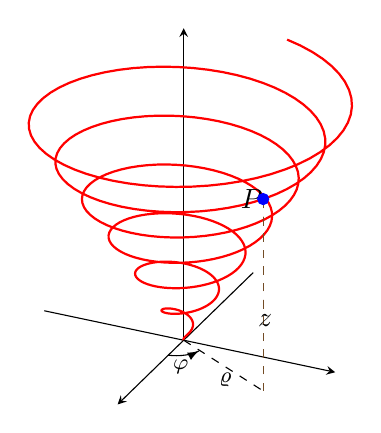
\begin{tikzpicture}
	\begin{axis}[
			view       = {-25}{-25},
			axis lines = middle,
			zmax       = 60,
			height     = 8cm,
			xtick      = \empty,
			ytick      = \empty,
			ztick      = \empty
		]
		\addplot3+ [
			ytick      = \empty,
			yticklabel = \empty,
			domain     = 0:14.7*pi,
			samples    = 400,
			samples y  = 0,
			mark       = none,
			thick,
			red,
		]
		( {x*sin(0.28*pi*deg(x))},{x*cos(0.28*pi*deg(x)},{x});
		\addplot3+ [
			mark options = {color=blue},
			mark         = *
		]
		coordinates {({\Point*sin(0.28*pi*deg(\Point))},
				{\Point*cos(0.28*pi*deg(\Point)}, {\Point})};
		\addplot3+ [
			domain    = 0:12*pi,
			samples   = 100,
			samples y = 0,
			mark      = none,
			dashed,
		]
		( {\Point*sin(0.28*pi*deg(\Point))}, {\Point*cos(0.28*pi*deg(\Point)}, {x} );
		\addplot3[
			mark=none,
			dashed
		]
		coordinates {(0,0,0) ({\Point*sin(0.28*pi*deg(\Point))},
				{\Point*cos(0.28*pi*deg(\Point)}, {0})};
		\draw[
			radius = 80,
			decoration = {
					markings,
					mark= at position 0.99 with {\arrow{latex}}
				},
			postaction=decorate
		]
		(axis cs:0,10,0) arc[start angle=80,end angle=14] (axis cs:14,0,0);
		\node at (axis cs:20,0,30) {$P$};
		\node at (axis cs:24,0,7) {$z$};
		\node [font=\footnotesize] at (axis cs:20,17,0) {$\varrho$};
		\node [font=\footnotesize] at (axis cs:6,15,0) {$\varphi$};
	\end{axis}
\end{tikzpicture}
\end{document}
